\documentclass[times, utf8, diplomski]{fer}
\usepackage{booktabs}
\usepackage{fixltx2e}
\begin{document}

% TODO: Navedite broj rada.
\thesisnumber{000}

% TODO: Navedite naslov rada.
\title{Obrada i analiza govora na ugradbenom računalnom sustavu u stvarnom vremenu}

% TODO: Navedite vaše ime i prezime.
\author{Paula Franić}

\maketitle

% Ispis stranice s napomenom o umetanju izvornika rada. Uklonite naredbu \izvornik ako želite izbaciti tu stranicu.
\izvornik

% Dodavanje zahvale ili prazne stranice. Ako ne želite dodati zahvalu, naredbu ostavite radi prazne stranice.
\zahvala{}

\tableofcontents
\listoffigures
\chapter{Uvod}
Digitalna obrada signala (DSP) svoj početak zabilježila je razvojem prvih digitalnih računala 60-ih i 70-ih godina prošlog stoljeća. Naravno, takva računala su bila izrazito skupa tako da se i primjena obrade signala koristila isključivo u vojne svrhe, medicini te razvoju radara i sonara, točnije u svrhe koje su ovisile o velikim financijskim ulaganjima.

Napretkom razvoja digitalnih računala, DSP je svoje uporište našao u razvoju komercijalnih proizvoda kakve danas poznajemo. Tako smo danas upoznati s digitalnim uređajima za obradu zvuka, slike, videa i slično.

Prije daljnje rasprave o digitalnoj obradi signala, razjasnit će se zašto se ona smatra posebnim područjem u inženjerstvu jest što obrađuje jedinstvenu vrstu podataka: signale. Signali su podatak koji najčešće dolazi iz prirode. Tako se njihovom obradom pokušava manipulirati kako bi se postigli ciljevi poput: poboljšanja kvalitete slike, kvalitete zvuka, videa,izdvajanje određenih značajki signala za potrebe raspoznavanja te kompresija.

U ovom radu fokusirat ćemo se na digitalnu obradu zvuka, točnije govora. Zvuk je longitudinalni val koji se vibracijama širi po prostoru, organ koji ga percipira jest uho. 

Tako ćemo kroz rad proći osnovni dio vezan uz anatomiju uha kako bismo mogli razjasniti koncept uređaja koji akvizira zvuk te ga obrađuje, specifikacije potrebnih komponenti za akviziciju i obradu zvuka (mikrofon, A/D pretvornik, mikrokontroler) te će fokus biti na implementaciji dogotalne obrade govora na ugradbenom računalnom sustavu u stvarnom vremenu.

\chapter{Analiza govora}
\section{Nastanak glasa}
Glas nastaje izbacivanjem zraka iz pluća koji putem grkljana, dolazi do glasnica. Prolaskom zraka kroz glasnice one vibriraju pa na taj način nastaje glas. Nakon prolaska glasa kroz glasnice, ono ulazi u ždrijelo te u usnu i nosnu šupljiu gdje se ton glasa mijenja te oblikuje. U oblikovanju glasova sudjeluje jezik, zubi, usne, nepce i čeljust.
Kod oblikovanja nastalog glasa, bitno je poznavati funkciju vokalnog trakta. Vokalni trakt se u širem smislu sastoji od sljedećih osnovnih dijelova:
\begin{itemize}
\item prostor izmedu glasnica, glottis
\item pharynx ili ždrijelo (veza usta i jednjaka)
\item usna šupljina
\item jezik
\item stražnje (meko) nepce
\item srednje nepce
\item prednje (tvrdo) nepce
\item nadzubno meso
\item zubi
\item usne
\item velum ili resica zatvara usnu šupljinu prema nosnoj
\item nosna šupljina koja završava s nosnicama
\end{itemize}
Vokalni trakt se ponaša kao svojevrstan filtar, koji će spektralno obojiti pobudni signal. Slično kao što se geometrijom cijevi kod orgulja određuje ton (visina i spektralni sastav) signala koji se formira, tako ce i geometrijski oblik vokalnog trakta određivati koje se spektralne komponente signala pojačavaju, a koje prigušuju.


\begin{figure}[hbt!]
 \centering
 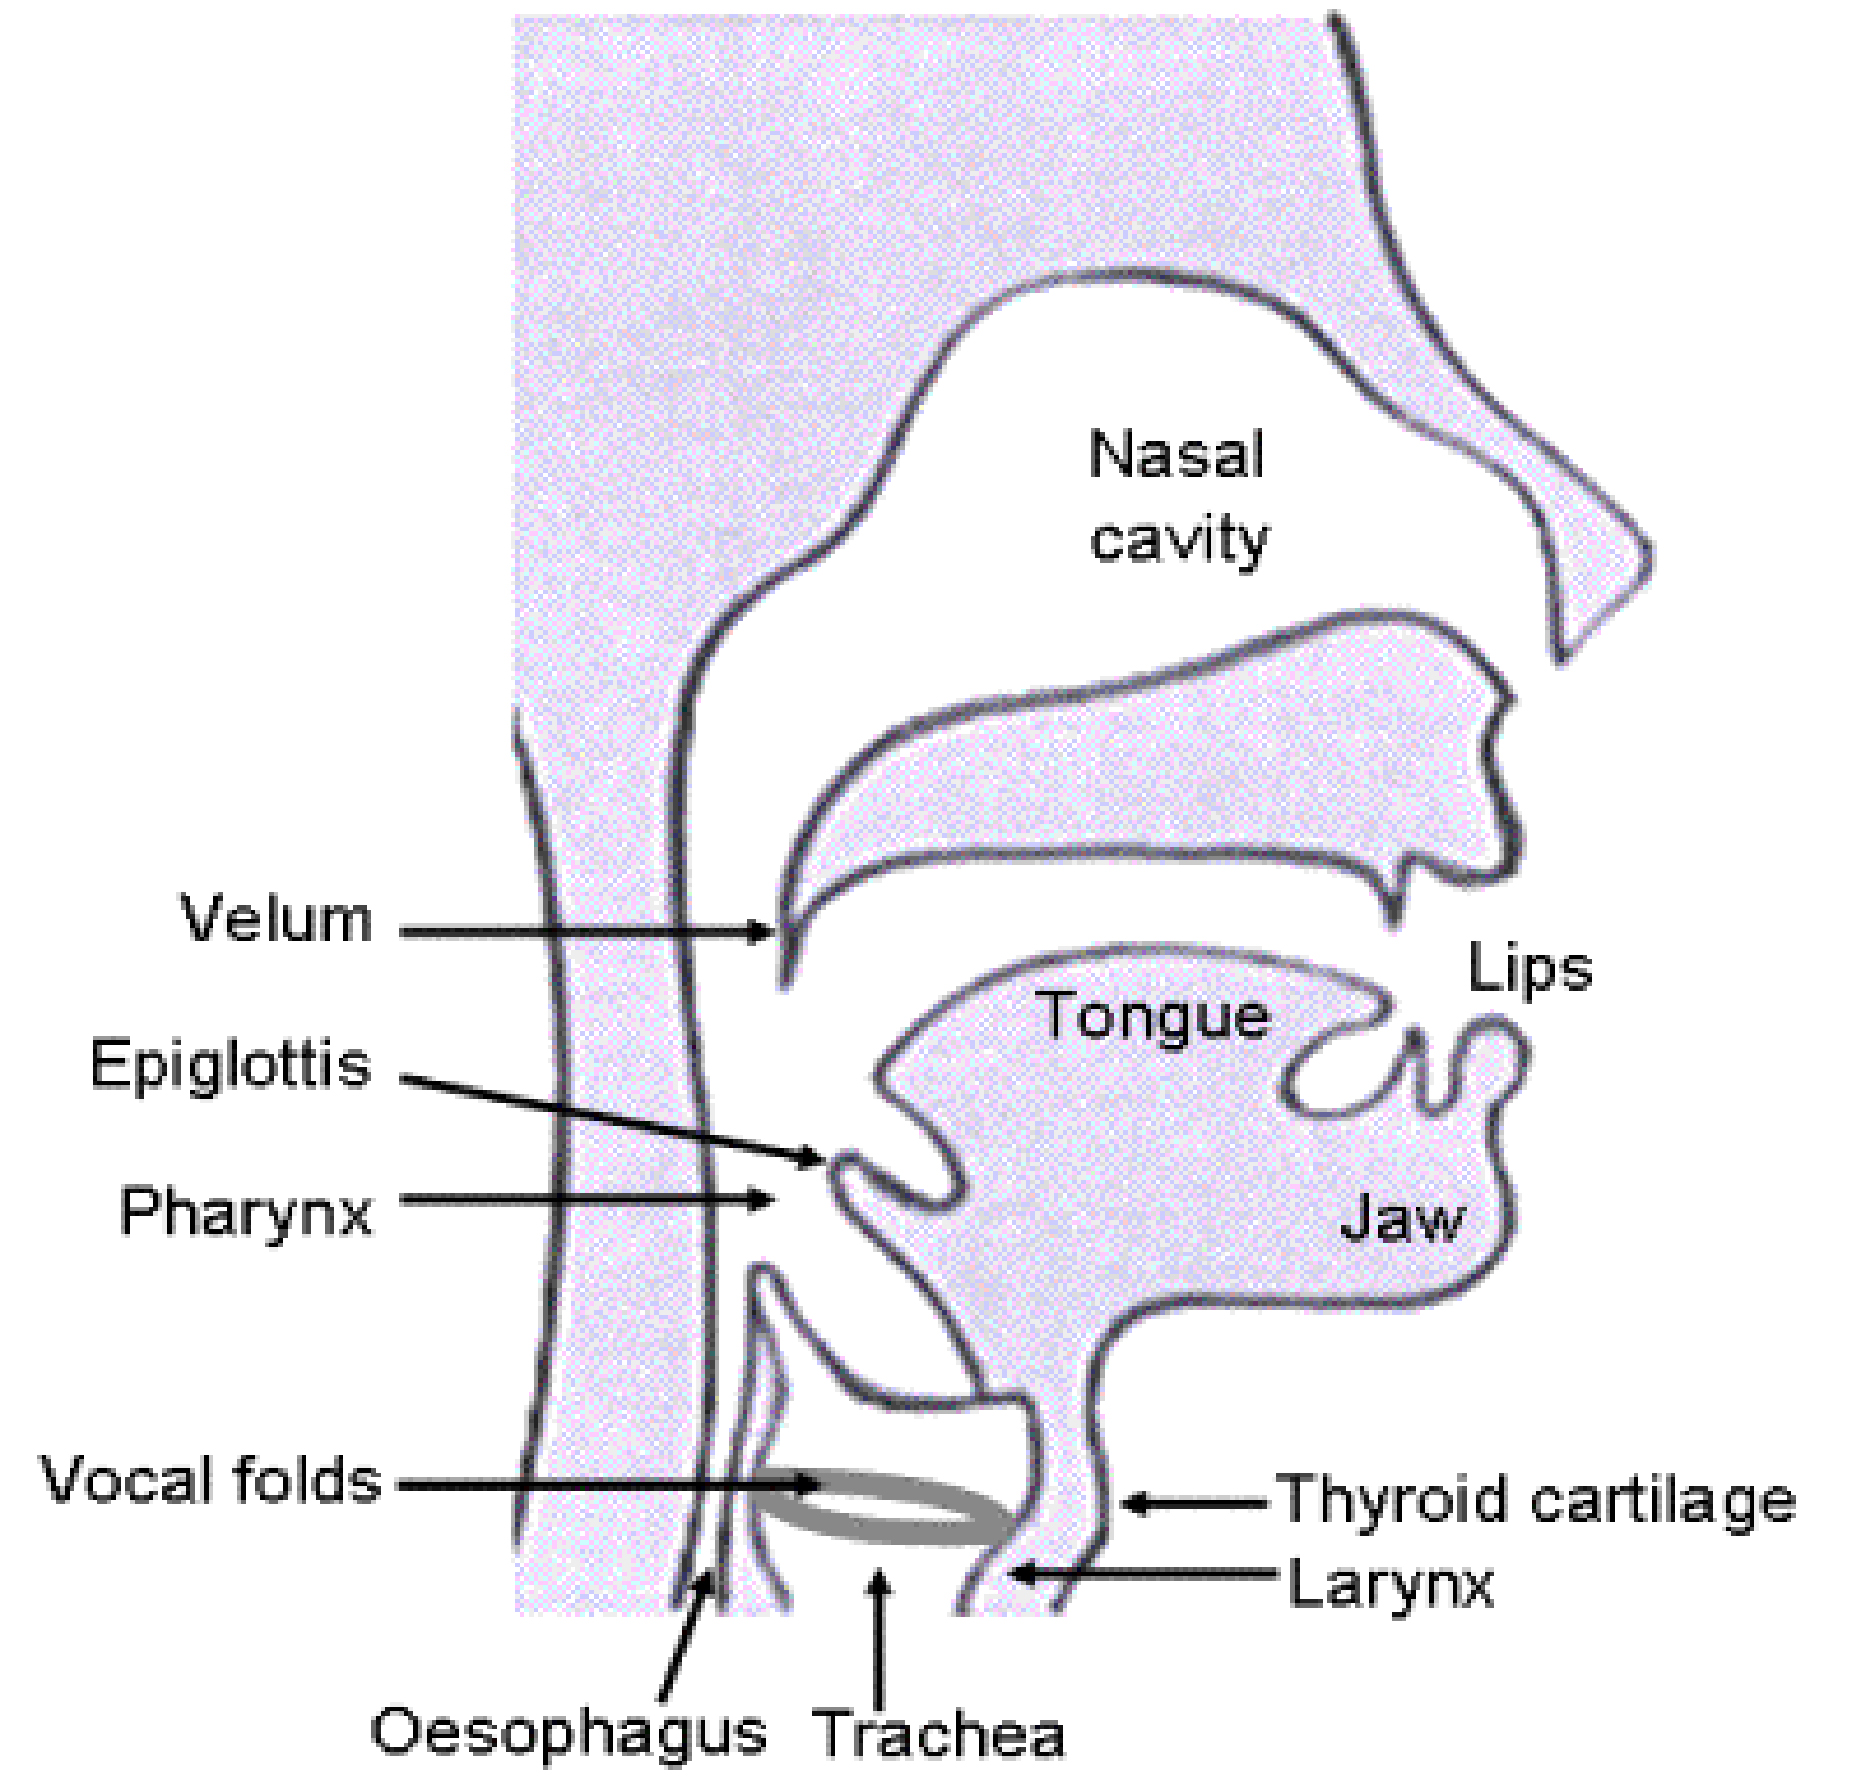
\includegraphics[scale=0.5]{photos/vokalni trakt.jpg}
 \caption{Anatomija ljudskog vokalnog trakta}
 \label{trakt}
\end{figure}

\section{Karakteristike glasa}
Ljudski glas je jedini koji može istovremeno proizvesti riječ i ton. Osnovne karakteristike glasa su: visina, intenzitet i boja. Dotaknut ćemo se i formanata jer njihovo postojanje uvelike utječe na frekvencijsku karakteristiku vokalnog trakta. 

\subsection{Visina glasa}
Visina glasa (ton) je perceptivni fenomen, a ovisi o fundamentalnoj frekvenciji koja je fizikalni parametar. Fundamentalna frekvencija (u daljnjem tekstu $F_{0}$) je broj vibracija koje glasnice proizvedu u jednoj sekundi. Što je veći broj vibracija glasnica, viša je vrijednost fundamentalne frekvencije pa i glas doživljavamo višim. Brzina titranja glasnica ovisi o debljini, dužini i napetosti glasnica, te o tlaku zraka koji prolazi između glasnica. Povišenje tlaka zraka dovodi istovremeno do povećanja intenziteta glasa i višeg tona. Na vrijednost $F_{0}$ utječu dob, spol, tjelesna konstitucija, socijalno okruženje, emocije, intelektualni status. Prosječna $F_{0}$ muškog glasa iznosi oko 120 Hz, a ženskog 225 Hz. Istraživanja $F_{0}$ djece još su složenija zbog čimbenika rasta i razvoja pa su podaci nekompletni, no zna se da je $F_{0}$ prvog plača vrlo visoka i kreće se između 400 i 600 Hz. Porastom kronološke dobi djeteta $F_{0}$ pada. Tako npr. za dječake kronološke dobi 10,5 godina vrijednost $F_{0}$ iznosi oko 250 Hz.

\subsection{Intenzitet}
Intenzitet ili jakost glasa percipiramo kao glasnoću, a ovisi o amplitudi titranja glasnica, te o  subglotičkom tlaku zraka\footnote{Zračni tlak u plućnim alveolama}. Što su te vrijednosti više, veća je i jačina glasa. Intenzitet se izražava u decibelima (dB). Intenzitetski raspon od tek čujnog glasa do najglasnijeg koji pojedinac može izvesti iznosi i do 70 dB. Ovu razliku između pianissima i fortissima, tj. najmanje i najveće razine zvuka nekog izvora, nazivamo dinamikom.

\subsection{Boja glasa}
Boja glasa je karakteristika glasa koja čini glas prepoznatljivim za određenog sugovornika. To je perceptivni fenomen koji svaki glas čini jedinstvenim i neponovljivim. Nastaje kao rezultat rezonancije, tj. obrade, ili možda bolje, dorade zvuka na putu od glasnica do izgovora. Taj put je vokalni trakt, a čine ga rezonantne šupljine, ili kraće, rezonatori. Boja glasa ima stalnu i promjenjivu sastavnicu. Stalna ovisi o  nasljednim i stečenim anatomsko-fiziološkim karakteristikama, ali isto tako i o načinu uporabe organa za glasanje na što utječe i kulturno okruženje. Promjenjiva sastavnica boje glasa odnosi se na izražajnu mogućnost govornika. Nadalje, o boji glasa prosuđuje se s biološkog, psihološkog, kulturnog, estetskog i patološkog stajališta što potvrduje koliko je ova karakteristika glasa složena, a opisi i definicije katkad i vrlo različiti. Sinonim za boju glasa je timbar, a u angloameričkoj literaturi vokalna kvaliteta ili kvaliteta glasa što je, zapravo, i širi pojam. U tom kontekstu, glas se opisuje kao pun, voluminozan, kreštav, dahtav, nazalan, drhtav, napet, šuškav, pucketav, zvonak, taman, promukao i slično \citep{optimala}. 

\subsection{Formanti}
Ono što će nam također utjecati na frekvencijski spektar glasa je duljina vokalnog trakta (prije spomenuti faktor kod nastajanja glasa) te veličina otvora na glotisu i ustima. Tu je bitno upoznati se s formantima. Formanti su intenzitetski naglašeni dijelovi spektra nastali rezoniranjem šupljine izgovorom nekog glasa. Možemo uočiti što je veći odnos presjeka otvora i duljine vokalnog trakta to je formant viši. Obično kod analize glasova primjećujemo tri formanta. Drugi formant je viši u smislu što se suženje pomiče prema ustima te što je veći odnos presjeka i duljine vokalnog trakta.

Sve ove karakteristike određuju frekvencijski spektar glasa. Znamo da ljudsko uho čuje 20 Hz do 20 kHz. Niže frekvencije nose informacije o govoru, dok visoke frekvencije doprinose jasnoći govora. Vidimo na slici \ref{raspon} podjelu područja na tri glavne cjeline, niske, srednje i visoke frekvencije. Ova informacija je bitna kod spektralne analize glasova.

\begin{figure}[hbt!]
 \centering
 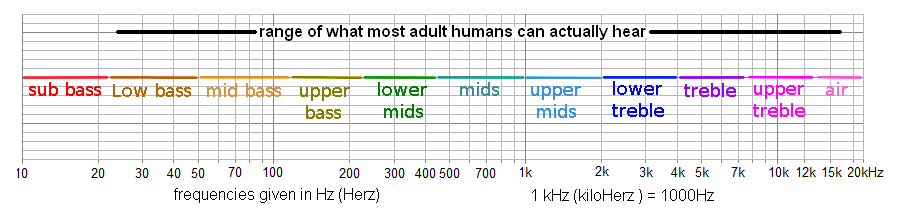
\includegraphics[scale=0.5]{photos/raspon.png}
 \caption{Raspon frekvencija}
 \label{raspon}
\end{figure}


\chapter{Analiza sluha}
\label{chap:sluh}
Nakon pojašnjenja nastanka te karakteristika govora, potrebno je objasniti rad organa za sluh i slušanje: uho.

Akvizicija zvuka počinje s vanjskim uhom. Kada je zvuk putuje prema vanjsko uhu, zvučni valovi, ili vibracije, putuju niz vanjski slušni kanal i udaraju u opnu (bubnjić). Bubnjić vibrira te se te vibracije zatim prenose na 3 sićušne kosti u srednjem uhu koje se nazivaju koščice (čekić, nakovanj i stremen). Koščice se ponašaju kao pojačalo zvuka. One zatim šalju zvučne valove u unutarnje uho i u slušni organ ispunjen tekućinom (pužnica).

\begin{figure}[hbt!]
 \centering
 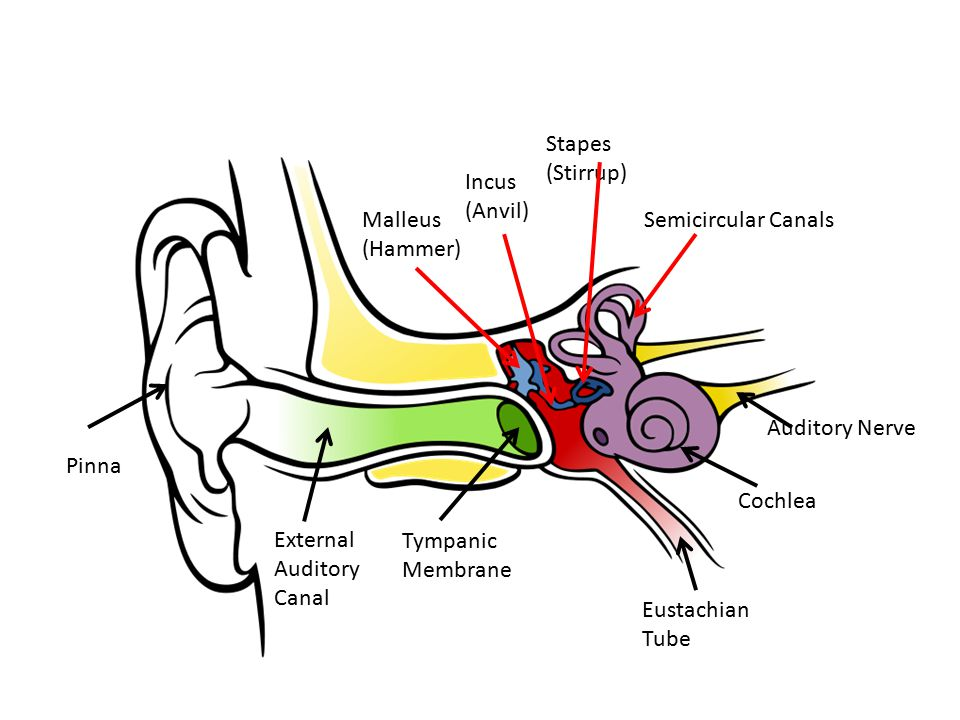
\includegraphics[scale=0.5]{photos/earanatomy.png}
 \caption{Anatomija uha }
\end{figure}

Kada zvučni valovi dosegnu unutarnje uho, oni se pretvaraju u električne impulse. Slušni živac šalje ove impulse u mozak. Mozak tada prevodi ove električne impulse kao zvuk.\citep{uho}

Jedna od bitnijih značajki uha jest što je ono, uz osjetilo vida, jedino osjetilo koje jačinu signala percipira po logaritamskoj skali. Znamo također da razlike u jačini snage između najtišeg i najglasnijeg zvuka koje ljudsko uho može percipirati jest 10\^6.

Također, prilikom obrade zvuka, moramo na umu imati da čovjek ima dva uha, tako da vrši akviziciju iz dva smjera te tako može percipirati smjer dolaska zvuka. Ovo nam je također bitno kod obrade kako bi imali dva izlaza koji simuliraju stereo zvuk.

Zanimljiva karakteristika uha jest ovisnost frekvencijskog odziva prema glasnoći zvuka, što možemo vidjeti na slici \ref{flemu}. Tu možemo uočiti nejednaku osjetljivost uha na niske frekvencije

\begin{figure}[hbt!]
 \centering
 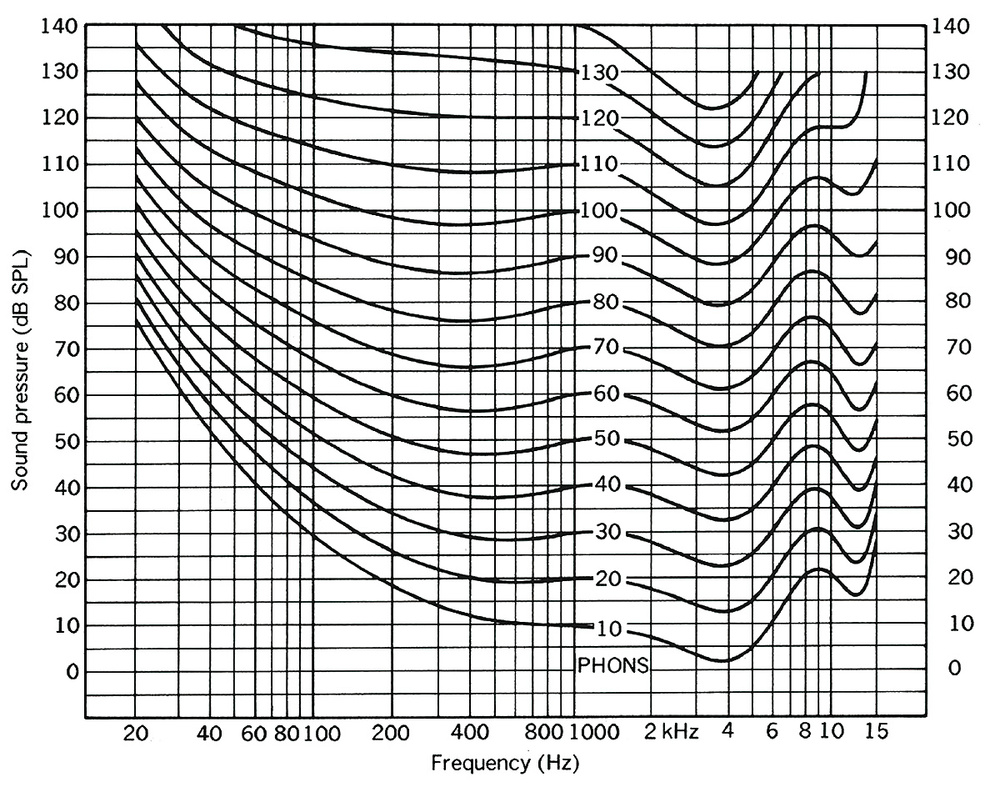
\includegraphics[scale=0.4]{photos/flemu.jpg}
 \caption{Fletcher-Munson krivulje}
 \label{flemu}
\end{figure}
Govor spada pod već spomenute zvučne signale. Kao što je u poglavlju \ref{chap:sluh} objašnjeno, ljudsko uho može percipirati signale frekvencija od 20 Hz do 20000 Hz. Ljudski govor spada u područje od 200 Hz do 5000 Hz, ovisno o spolu i dobi osobe. Iako je tu već očigledno da nam neće biti potreban spektar iznad 5000 Hz, nastojat ćemo ga zadržati nakon očitavanja kako ne bi gubili na kvaliteti signala, što nam je u ove svrhe bitno.

\chapter{Sustav za obradu i analizu govora}
Za razvoj sustava čija je svrha obrada i analiza govora koristi se MATLAB za generiranje filtarskih realizacija za obradu govora te STM32F4-Discovery ugradbeni sustav kojim će se vršiti akvizicija i filtracija signala.

\section{Izvedba filtarskih realizacija}
U poglavlju \ref{chap:sluh} smo se upoznali s činjenicom da je raspon ljudskog sluha od 20 Hz do 20000 Hz, no isto tako prilikom govora možemo primijetiti da se u tom rasponu kreće i frekvencijski spektar što znači da prilikom govora osobe, pogotovo djeca koja imaju prirodno viši glas, mogu generirati frekvencije i iznad 10000 Hz (prilikom izgovora glasa C). 

Tako je potrebno generirati 19 pojasno propusnih filtara  čiji su parametri usklađeni s međunarodnim standardima i preporukama (ISO R 266, DIN 401 i ANSI S1.6-1976) \citep{optimala}. 
Za realizaciju filtra se koristi Butterworth filtar. Ovakav tip digitalnog filtra proizišao je iz analogne realizacije britanskog inženjera Stephena Butherwortha kojeg je predstavio u svom članku "On the Theory of Filter Amplifiers". Glavna značajka ovog tipa filtra jest to što je on maksimalno gladak. To znači da je jednako osjetljiv za svaku frekvenciju ovisno o području propuštanja.

Butterworth filtar predstavlja IIR tip filtra (eng. \textit{infinite impulse response}). Izlaz IIR filtra ovisi o svom ulazu te je impulsni odziv ovakav:


$\sum_{l=0}^{N}a_{l}y[n-l] = \sum_{k=0}^{M}b_{k}x[n-k]$


gdje $N$ i $M$ predstavljaju broj uzoraka na ulazu i izlazu, slijedom.

Razlog zbog kojeg je korišten IIR tip filtra jest zbog svojeg dobrog gušenja nepropusnog dijela sa vrlo malim brojem filtarskih koeficijenata, za razliku od FIR filtra. Zašto je ovaj faktor iznimno bitan je zbog smanjenja vremena procesiranja signala. Na slici ... možemo vidjeti FIR i IIR

bikvadratne sekcije

\section{STM32F4-Discovery}

\subsection{Glavne značajke ugradbenog računalnog sustava}
Sustav koji želimo razviti za potrebe obrade govornog signala nam zahtjeva ključne komponente:

\begin{enumerate}
\item procesor sa DSP značajkama
\item analogno-digitalni pretvornik s performansama prilagođenim za audio signale
\item MEMS mikrofon koji vrši akviziciju signala
\end{enumerate}

Kod ovakvog sustava potrebno je pobrinuti se da je akvizicija signala brza i ne narušava inicijalnu frekvencijsku karakteristiku glasa te da je obrad signala brza i kvalitetna. 

Naš ugradbeni računalni sustav jest STM32F407VG. On sadrži ARM Cortex-M4 procesor sa DSP značajkama koji će nam biti ključan za daljnju obradu signala. Ovaj mikrokontroler već ima ugrađeni MEMS mikrofon i A/D pretvornik no oni su namijenjeni za opću primjenu, dok su nama potrebne komponente za isključivu obradu audio signala tako da će se u daljnjim potpoglavljima napraviti usporedba dostupnih te traženih komponenti.

\section{DSP Procesor}
\label{instr}
Odabrani ugradbeni računalni sustav sadrži ARM-ov procesor Cortex-M4. Ovaj procesor spada u familiju Cortex-M procesora koji se koriste za ovakve svrhe. Glavne karakteristike takvih procesora je visoka efikasnost potrošnje energije, mala površina procesora, kratki cjevovodi te rad na frekvenciji oko 200 MHz \citep{cortexm4}.

Ono što čini ovaj procesor pogodnim za digitalnu obradu audio signala jest što ima podršku za funkcije tog tipa pomoću SIMD i MAC instrukcija.

\textit{Single Instruction Multiple Data} (SIMD) je skupina instrukcija koje omogućuju paralelno izvođenje operacije za više podataka.

\begin{figure}[hbt!]
 \centering
 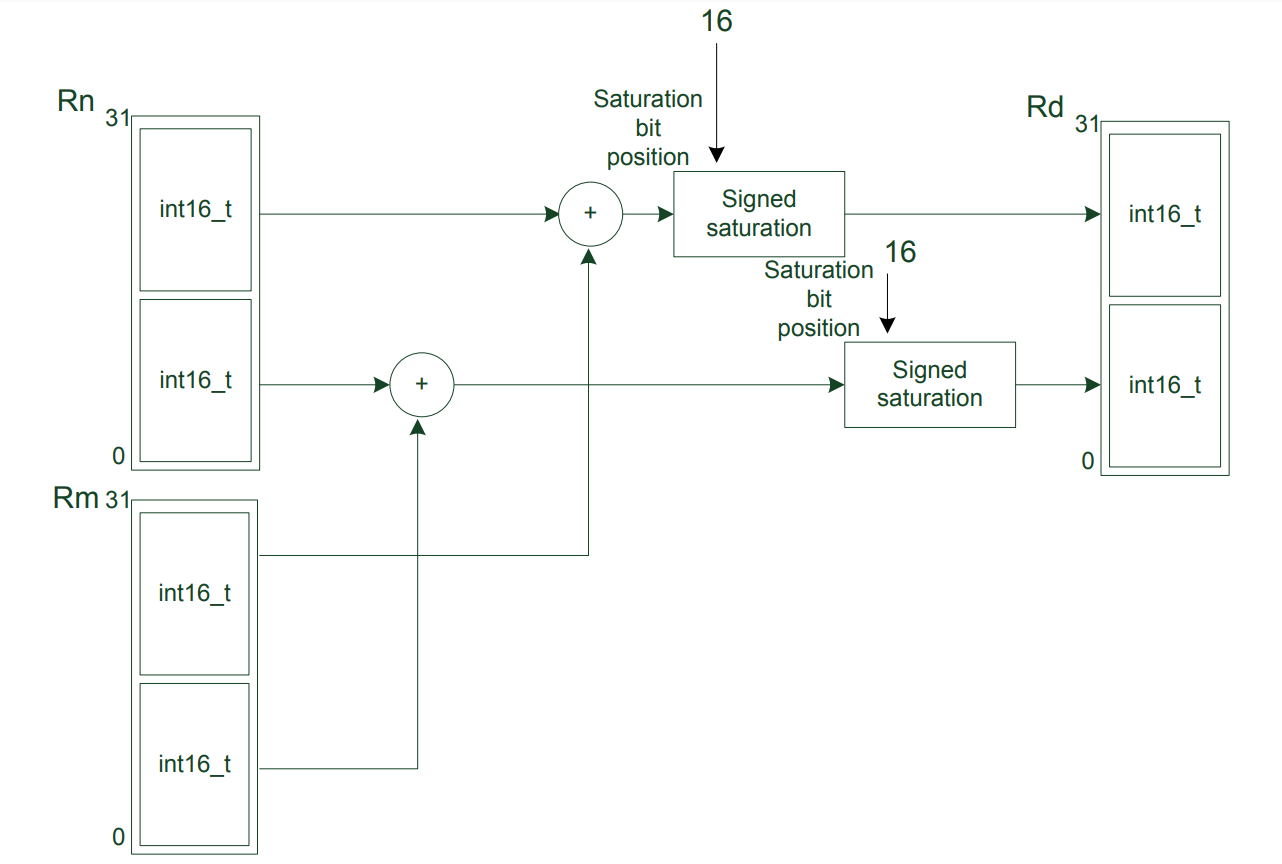
\includegraphics[scale=0.4]{photos/simd.png}
 \caption{Dijagram izvođenja SIMD instrukcije zbrajanja}
 \label{SIMD}
\end{figure}

Kao što se vidi na slici \ref{SIMD}, podatke koje želimo zbrojiti podijelimo na nižih 16 bita i viših 16 bita. Kod oba podatka zbrajaju se posebno niži bitovi i posebno viši bitovi. Ono što je ključno kod SIMD naredbe jest aritmetika zasićenja. U slučaju da zbroj nižih ili viših bitova prelazi maksimalni broj koji je moguće spremiti, on se zaokružuje na taj maksimalni broj. SIMD instrukcije zbog ove karakteristike imaju najčešću primjenu u audio sustavima.

\textit{Multiply and Accumulate} (MAC) je skupina instrukcija fundamentalna za digitalnu obradu signala. Ona omogućuje množenje dvaju podataka te zbrajanje s vrijednosti akumulatora u jednom ciklusu, što je čini savršenom kod filtriranja podataka pomoću FIR filtara.

$a <- a + x * y$

\subsection{CMSIS DSP biblioteka}
Za ugradbene sustave s Cortex-M procesorima postoji razvijena biblioteka za digitalnu obradu signala. Biblioteka je podijeljena na nekoliko funkcija od kojih svaka pokriva određenu kategoriju:

\begin{itemize}
\item Osnovne matematičke funkcije
\item Brze matematičke funkcije
\item Složene matematičke funkcije
\item Filtri
\item Matrične funkcije
\item Funkcije transformacije
\item Funkcije upravljanja motorom
\item Statističke funkcije
\item Funkcije podrške
\item Interpolacijske funkcije
\end{itemize}

Svaka od ovih funkcija ima podršku za 8-bitne, 16-bitne, 32-bitne \textit{integer} podatke te 32-bitne \textit{floating point} podatke.

Za potrebe filtracije će se koristiti kategorija funkcija filtri te se koriste 16-bitni podaci \textit{integer} vrijednosti kako bi se umanjila vremenska komponenta obrade signala. U središtu obrade signala će biti funkcija 

\textit{$arm\_biquad\_cascade\_df2T\_f32 (const arm\_biquad\_cascade\_df2T\_instance\_f32 *S, const float32\_t *pSrc, float32\_t *pDst, uint32\_t blockSize)$} 

koja koristi bikvadratne sekcije IIR filtra. Struktura koja omogućuje filtraciju signala jest Direktna II transponirana realizacija filtra. Na slici \ref{df2t} možemo vidjeti blok dijagram izvedbe strukture.

\begin{figure}[hbt!]
 \centering
 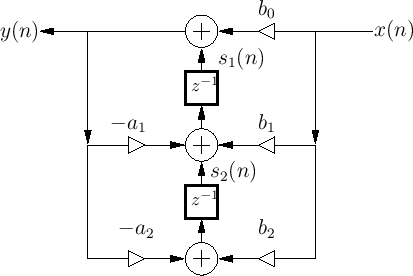
\includegraphics[scale=0.6]{photos/df2t.png}
 \caption{Direktna II transponirana realizacija filtra}
 \label{df2t}
\end{figure}

Složenost proračuna kod direktne II transponirane realizacije drugog reda (za bikvadratne sekcije) jest: 5 množenja, 4 dvoulazna zbrajanja i 2 memorijske lokacije. S obzirom da koristimo IIR butterworth filtar sa sedam koefijenata, imamo 2?? bikvadratne sekcije te tipe imamo sveukupno 10 množenja, 8 dvoulaznih zbrajanj te 4 memorijske lokacije za stanja. Ako usporedimo sa FIR relizacijom filtra i uzmemo u obzir 40 filtarskih koeficijenata da bi postigli jednake performanse kao i IIR filtar, imamo sveukupno: 40 množenja, 1 zbrajanje te nemamo memorijskih lokacija.


S obzirom da se radi o Cortex-M4 procesoru koji ima podršku za MAC i SIMD instrukcije koje su objašnjene u poglavlju \ref{SIMD}, procesno vrijeme se dvostruko?? ubrzava s obzirom da - nema spominjanja korištenja takvih instrukcija kod iir filtara
\section{Vanjske komponente}
\subsection{MEMS mikrofon}

\chapter{Napredna obrada digitalnog signala}
\chapter{Algoritam višepojasnog filtriranja}
\section{Audio kodek}
Za potrebe akvizicije i obrade signala, koristi se STM-ov razvijeni kodek. Kodek definira potrebne protokole za komunikaciju sa mikrofonom, slanje signala na obradu te pomoću DMA reprodukciju signala na izlazu. Za potrebe razumijevanja aplikacije, razjasnit će se komunikacija mikrofon - procesor te procesor - izlaz (zvučnik ili slušalice).

\subsection{Komunikacija mikrofon - kodek}
Ova komunikacija je omogućena putem I2S protokola. I2S protokol podržava komunikaciju u slučaju prijenosa audio signala. Ovaj protokol spada pod SPI protokol (engl. \textit{serial peripheral interface}). Takvi protokoli definiraju komunikaciju uređaj sa perifernim komponentama, u ovom slučaju s mikrofonom, te definiraju koji uređaj vodi komunikaciju (engl. \textit{master}) i koji sluša (engl. \textit{slave}).

Ono što je potrebno definirati koji uređaj vodi komunikaciju, a taj uređaj će davati \textit{slaveu} \textit{clock} koji određueje brzinu prijenosa podataka koji također moramo omogućiti u konfiguraciji. Zatim definiramo frekvenciju uzorkovanja koja će u našem slučaju biti 44.1 kHz. Naravno, da bi \textit{master} znao kojem uređaju šalje \textit{clock}, inicijaliziraju se i GPIO jedinice koje to omogućuju. Na taj način su uređaji usklađeni te mogu početi s komunikacijom.  

\subsection{Komunikacija kodek - izlaz}
Za potrebe komunikacije 


\subsection{PDM filtar}
S obzirom da se koristi MEMS mikrofon koji daje digitalni izlaz u obliku PDM-a (engl.\textit{pulse density modulation}), takav izlaz je potrebno pretvoriti u informaciju koja se može čitati na izlazu, a to je zvuk u obliku PCM-a (engl. \textit{pulse code modulation})

\chapter{Analiza performansi sustava}
\chapter{Zaključak}
Zaključak.

\bibliography{literatura}
\bibliographystyle{fer}

\begin{sazetak}
Sažetak na hrvatskom jeziku.

\kljucnerijeci{Ključne riječi, odvojene zarezima.}
\end{sazetak}

% TODO: Navedite naslov na engleskom jeziku.
\engtitle{Title}
\begin{abstract}
Abstract.

\keywords{Keywords.}
\end{abstract}

\end{document}
